
        \documentclass[addpoints,spanish, 12pt,a4paper]{exam}
        %\documentclass[answers, spanish, 12pt,a4paper]{exam}
        
        %\printanswers
        \pointpoints{punto}{puntos}
        \hpword{Puntos:}
        \vpword{Puntos:}
        \htword{Total}
        \vtword{Total}
        \hsword{Resultado:}
        \hqword{Ejercicio:}
        \vqword{Ejercicio:}

        \usepackage[utf8]{inputenc}
        \usepackage[spanish]{babel}
        \usepackage{eurosym}
        %\usepackage[spanish,es-lcroman, es-tabla, es-noshorthands]{babel}

        \usepackage{pgf,tikz}

        \usepackage[margin=1in]{geometry}
        \usepackage{amsmath,amssymb}
        \usepackage{multicol, xparse}

        \usepackage{yhmath}
        \usepackage{pdflscape}

        \usepackage{verbatim}
        %\usepackage{pstricks}


        \usepackage{graphicx}
        \graphicspath{{../img/}}




        \let\multicolmulticols\multicols
        \let\endmulticolmulticols\endmulticols
        \RenewDocumentEnvironment{multicols}{mO{}}
         {%
          \ifnum#1=1
            #2%
          \else % More than 1 column
            \multicolmulticols{#1}[#2]
          \fi
         }
         {%
          \ifnum#1=1
          \else % More than 1 column
            \endmulticolmulticols
          \fi
         }
        \renewcommand{\solutiontitle}{\noindent\textbf{Sol:}\enspace}

        \newcommand{\samedir}{\mathbin{\!/\mkern-5mu/\!}}

        \newcommand{\class}{4ºESO - Académicas}
        \newcommand{\examdate}{\today}

        %\newcommand{\tipo}{A}


        \newcommand{\timelimit}{50 minutos}

        \renewcommand{\solutiontitle}{\noindent\textbf{Solución:}\enspace}


        \pagestyle{head}
        \firstpageheader{
\includegraphics[width=0.2\columnwidth]{header_left}}{\textbf{Departamento de Matemáticas\linebreak \class}\linebreak \examnum}{
\includegraphics[width=0.1\columnwidth]{header_right}}
        \runningheader{\class}{\examnum}{Página \thepage\ of \numpages}
        \runningheadrule
        
        \pointsinrightmargin % Para poner las puntuaciones a la derecha. Se puede cambiar. Si se comenta, sale a la izquierda.
        \extrawidth{-2.4cm} %Un poquito más de margen por si ponemos textos largos.
        \marginpointname{ \emph{\points}}

        
            \newcommand{\tipo}{A}\newcommand{\examnum}{Examen Global}
            
            
        \DeclareUnicodeCharacter{2212}{-}
        
        \begin{document}
        \noindent
        % \begin{tabular*}{\textwidth}{l @{\extracolsep{\fill}} r @{\extracolsep{6pt}} }
        % \textbf{Nombre:} \makebox[3.5in]{\hrulefill} & \textbf{Fecha:}\makebox[1in]{\hrulefill} \\
        %  & \\
        % \textbf{Tiempo: \timelimit} & Tipo: \tipo 
        % \end{tabular*}
        % \rule[2ex]{\textwidth}{2pt}
        % Esta prueba tiene \numquestions\ ejercicios. La puntuación máxima es de \numpoints. 
        % La nota final de la prueba será la parte proporcional de la puntuación obtenida sobre la puntuación máxima. 
\begin{center}

\begin{tabular*}{\textwidth}{l @{\extracolsep{\fill}} r @{\extracolsep{6pt}} }
\textbf{Nombre:} \makebox[3.5in]{\hrulefill} & \textbf{Fecha:}\makebox[1in]{\hrulefill} \\
 & \\
\textbf{Tiempo: \timelimit} & Tipo: \tipo 
\end{tabular*}
\rule[2ex]{\textwidth}{2pt}        
\textbf{Instrucciones:} \begin{itemize}
\item \textbf{Si solo tienes una evaluación pendiente:} Tienes que hacer \textbf{todos} los ejercicios del bloque correspondiente a la evaluación, incluido el "postre". (5 ejercicios en total). \textbf{Tiempo: 50 minutos}
\item \textbf{Si tienes más de una pendiente:} Tienes que hacer \textbf{los dos primeros} ejercicios de cada evaluación. (6 ejercicios en total). \textbf{Tiempo: 50 minutos}
\item \textbf{Si tienes todo aprobado} tienes que hacer de cada evaluación el \textbf{último ejercicio o ejercicio "postre"} y otro a elegir. (6 ejercicios en total) \textbf{Tiempo: 50 minutos}
\end{itemize}
\rule[2ex]{\textwidth}{2pt}
\end{center}

        
        
        
% \rule[2ex]{\textwidth}{2pt}
%       
%        \begin{center}
%
%
%        \addpoints
%             %\gradetable[h][questions]
%            \pointtable[h][questions]
%        \end{center}
%
%        \noindent
% \rule[2ex]{\textwidth}{2pt}

        \begin{questions}

%        \question Calcula los siguientes límites:
%        \begin{multicols}{1}
%        \begin{parts} \part[1] $$\lim_{x \to 3}\left(\frac{3 x^{2} - 11 x + 6}{x^{3} - 3 x^{2} + x - 3}\right)$$  \begin{solution}   $\frac{7}{10}$   \end{solution} \part[1] $$\lim_{x \to \infty} e^{1 - x}$$  \begin{solution}   $0$   \end{solution} \part[1] $$\lim_{x \to -2}\left(\frac{x^{3} + x^{2} - x + 2}{x^{2} + 4 x + 4}\right)$$  \begin{solution}   No existe el límite   \end{solution} \part[2] $$\lim_{x \to 2} \left(\frac{x^{3} - 4}{x^{2}}\right)^{\frac{1}{x - 2}}$$  \begin{solution}   $e^{2}$   \end{solution}
%        \end{parts}
%        \end{multicols}
\section*{1ª Evaluación}        
		\question[1] Calcula
		\begin{parts}
		\part Racionaliza y simplifica: $\dfrac{2+\sqrt{2}}{2-\sqrt{2}}$
\begin{solution} $2 \sqrt{2} + 3 $ \end{solution}
		%\part Racionaliza y simplifica:  $\dfrac{\sqrt{3}}{2\sqrt{3}-\sqrt{2}}$ \begin{solution} $=\dfrac{\sqrt{3}\cdot\left(2\sqrt{3}+\sqrt{2}\right)}{\left(2\sqrt{3}-\sqrt{2}\right)\left(2\sqrt{3}+\sqrt{2}\right)}=\dfrac{6\sqrt{6}}{12-2}=\dfrac{6\sqrt{6}}{10}$ \end{solution}


%\part[] Racionaliza y simplifica:  $\dfrac{\sqrt{5}}{2\sqrt{5}+\sqrt{2}}$\begin{solution} $\frac{10 - \sqrt{10}}{18}$ \end{solution}
%\part[] Racionaliza y simplifica:  $\dfrac{\sqrt{5}}{3\sqrt{5}+\sqrt{3}}$\begin{solution} $\frac{15 - \sqrt{15}}{42}$ \end{solution}

%\part[] Aplica la definición de logaritmo para calcular: $\log_4 \sqrt{0,25}$\begin{solution} $\to 4^x=\sqrt{\frac{1}{4}}\to4^x=4^{-1/2}\to\log_4 \sqrt{0,25}=-\frac{1}{2}$ \end{solution}
%\part[1] Aplica la definición de logaritmo para calcular: $\log_{4}{\sqrt{0,125}}$\begin{solution} $- \frac{3}{4}$ \end{solution}
%\part[1] Aplica la definición de logaritmo para calcular: $\log_5 \sqrt[3]{25}$\begin{solution} $\to 5^x=\sqrt[3]{5^2}\to5^x=5^{2/3}\to\log_5 \sqrt[3]{25}=\frac{2}{3}$ \end{solution}
%\part Aplica la definición de logaritmo para calcular: $\log_4 \sqrt[3]{16}$\begin{solution} $\frac{2}{3}$ \end{solution}
%\part[2] Sabiendo que $\log x=1$ y $\log y=-2$, calcula: $\log (\dfrac{100\cdot x^2}{\sqrt{x\cdot y}})$\begin{solution}$\log (\frac{100\cdot x^2}{\sqrt{x\cdot y}})=\frac{3 \log{\left (x \right )}}{2} - \frac{\log{\left (y \right )}}{2} + 2=2 - \frac{-2}{2} + \frac{3 \cdot 1}{2}=\frac{9}{2}$      \end{solution}
\part Aplica la definición de logaritmo para calcular: $\log_4 \sqrt{0,25}$
\begin{solution} $\to 4^x=\sqrt{\frac{1}{4}}\to4^x=4^{-1/2}\to\log_4 \sqrt{0,25}=-\frac{1}{2}$ \end{solution}
\part Sabiendo que $\log x=2$ y $\log y=-1$, calcula: $\log (\dfrac{\sqrt{x\cdot y}}{100\cdot x^2})$
\begin{solution}
$\log (\frac{\sqrt{x\cdot y}}{100\cdot x^2})=\frac{3 \log{\left (x \right )}}{2} - \frac{\log{\left (y \right )}}{2} + 2=2 - \frac{-1}{2} + \frac{3 \cdot 2}{2}=\frac{11}{2}$      
\end{solution}
\end{parts}



\question[1] Resuelve las siguientes ecuaciones: 

		\begin{parts}
		\part $$2+\sqrt{2x+3}=2x-1$$\begin{solution}$2+\sqrt{2x+3}=2x-1 \to x=3$ \end{solution}
		\part $$3^{x-1}+3^{x}+3^{x+1}=117$$\begin{solution}$3^{x-1}+3^{x}+3^{x+1}=117 \to x=3$ \end{solution}	
		\end{parts}
%
%\question[1] Resuelve las siguientes ecuaciones: 
%		\begin{parts}
%\part $$\sqrt{x+3}+\sqrt{x-2}=5$$
%\begin{solution}$\sqrt{x+3}+\sqrt{x-2}=5 \to x=6$ \end{solution}
%
%\part $$2^{x^2-4x+1}=\frac{1}{4}$$
%\begin{solution}$2^{x^2-4x+1}=\frac{1}{4} \to x=1, x=3$ \end{solution}
%
%		\end{parts}


%\question[1] Halla el valor de \emph{k} para que la siguiente división sea exacta: $(3x^2+kx-2):(x+2)$
%\begin{solution} $\to 10-2k=0 \to k=5 $ \end{solution}



\question[1] Halla el valor de \emph{k} para que $3x^2+kx-2$ sea divisible por $x+2$
\begin{solution} $\to 10-2k=0 \to k=5 $ \end{solution}

\addpoints

%\question[1] Simplifica la fracción algebraica: $$\dfrac{2x^3-5x^2+3x}{2x^2+x-6} $$
%\begin{solution}$=\dfrac{2x\left(x-1\right)\left(x-\dfrac{3}{2}\right)}{2\left(x+2\right)\left(x-\dfrac{3}{2}\right)}=\dfrac{x(x-1)}{x+2}$  \end{solution}
%
%\question[1] Simplifica la fracción algebraica: $$\frac{2 x^{3} + 2 x^{2} - 4 x}{3 x^{4} + 3 x^{3} - 6 x^{2}}$$
%\begin{solution} $\frac{2 x^{3} + 2 x^{2} - 4 x}{3 x^{4} + 3 x^{3} - 6 x^{2}}=\frac{2 x \left(x - 1\right) \left(x + 2\right)}{3 x^{2} \left(x - 1\right) \left(x + 2\right)}=\frac{2}{3 x}$  \end{solution}

\question[1] Simplifica la fracción algebraica: $$\frac{3 x^{4} - 3 x^{3} - 6 x^{2}}{2 x^{3} - 2 x^{2} - 4 x}$$
\begin{solution} $\frac{3 x^{4} - 3 x^{3} - 6 x^{2}}{2 x^{3} - 2 x^{2} - 4 x}=\frac{3 x^{2} \left(x - 2\right) \left(x + 1\right)}{2 x \left(x - 2\right) \left(x + 1\right)}=\frac{3 x}{2}$  \end{solution}

%


        \question[1] \textbf{Ejercicio "postre":} Indica a cuáles de los conjuntos
$\mathbb{N}$ (naturales), $\mathbb{Z}$ (enteros), $\mathbb{Q}$ (racionales), $\mathbb{R}$ (reales) pertenecen cada uno de los siguientes números:
\begin{center}
\begin{tabular}{|c |c |c |c |c|}\hline
&$\mathbb{N}$& $\mathbb{Z}$& $\mathbb{Q}$&$\mathbb{R}$\\ 
\hline
$\frac{8}{16}$&&&&\\
\hline
$\sqrt[3]{-27}$&&&&\\
\hline
$3.0\wideparen{1}$&&&&\\
\hline
$-\frac{12}{4}$&&&&\\
\hline
$-\sqrt{25}$&&&&\\
\hline
$\sqrt{8}$&&&&\\
\hline
$4$&&&&\\
\hline
$\pi$&&&&\\
\hline
$\sqrt{-4}$&&&&\\
\hline
$\frac{39}{13}$&&&&\\
\hline
\end{tabular}

\end{center}


        


\section*{2ª Evaluación}

%\question[1] El área de un rectángulo no variaría si se aumentase su base en 6 cm y a la vez se disminuyese su altura en 3 cm. Tampoco variaría si la base disminuyese en 4 cm y la altura aumentase en 3 cm. ¿Cuáles son las dimensiones actuales del rectángulo?\begin{solution} $\left\{\begin{matrix}xy=(x+6)(y-3) \\ xy=(x-4)(y+3)\end{matrix}\right. \to  x = 24, \  y = 15 \to $ Base 24 cm y altura 15 cm \end{solution}

\question[1] Si se aumenta la base de un rectángulo en 4 cm y se disminuye la altura en 2 cm se tiene la misma área; en cambio, si la base se disminuye en 10 cm y se aumenta la altura en 10 cm, entonces el área es 40 cm2 menor. Averigua las dimensiones del rectángulo.\begin{solution} $\left\{\begin{matrix}(x+4)(y-2)=xy \\ (x-10)(y+10)=xy-40\end{matrix}\right. \to  x = 16, \  y = 10 \to $ Base 16 cm y altura 10 cm \end{solution}


 \question[1] Contesta a las siguientes cuestiones:\begin{parts} 
 \part  Resuelve $\dfrac{x^{2} - 4}{x^{2} - 9} \geq  0$\begin{solution} $\left(-\infty, -3\right) \cup \left[-2, 2\right] \cup \left(3, \infty\right)$\end{solution} 
%  \part Resuelve $\dfrac{x^{2} -4x +4}{x^{2} - 1} \geq  0$\begin{solution} $\left(-\infty, -1\right) \cup \left(1, \infty\right)$\end{solution} 
 % \part Resuelve $\dfrac{x^{2} - 4}{x^{2} - 9} \leq  0$\begin{solution} $\left(-3, -2\right] \cup \left[2, 3\right)$\end{solution}
 \part Calcula el dominio de: $f(x)=\sqrt{x^2+3x+2}$\begin{solution} $\left(-\infty, -2\right] \cup \left[-1, \infty\right)$\end{solution}
 %\part Calcula el dominio de: $f(x)=\dfrac{2x-1}{x^{2} + 4 x + 3}$\begin{solution} $\left(-\infty, -3\right) \cup \left(-3, -1\right) \cup \left(-1, \infty\right)$\end{solution}
  
 \end{parts} 
 
\question[1] Representa la siguiente función a trozos e indica sus propiedades:
%\begin{parts} \part[1] $f(x)=\begin{cases} 2 x + 2 & \text{for}\: x \leq -1 \\x^{2} - 2 x & \text{otherwise} \end{cases}$\begin{solution} \scalebox{.6}{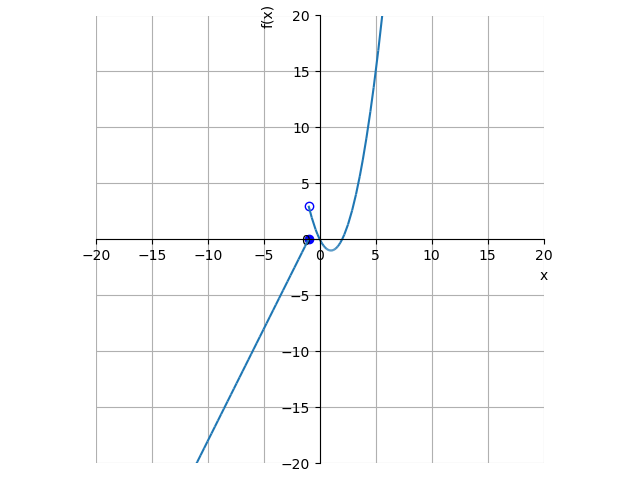
\includegraphics[width=1\columnwidth]{ex_funcion_a_trozos_0}}\end{solution} \part[1] $f(x)=\begin{cases} 3 - 2 x & \text{for}\: x < 1 \\x^{2} - 6 x + 8 & \text{otherwise} \end{cases}$\begin{solution} \scalebox{.6}{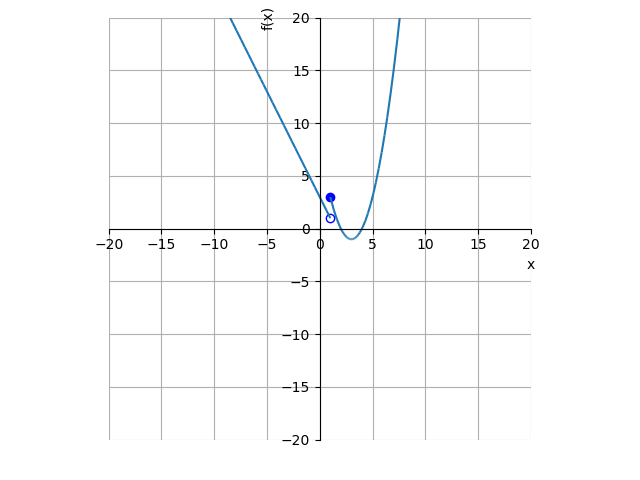
\includegraphics[width=1\columnwidth]{ex_funcion_a_trozos_1}}\end{solution} \part[1] $f(x)=\begin{cases} 2 x - 3 & \text{for}\: x \leq -1 \\- x^{2} + 2 x & \text{otherwise} \end{cases}$\begin{solution} \scalebox{.6}{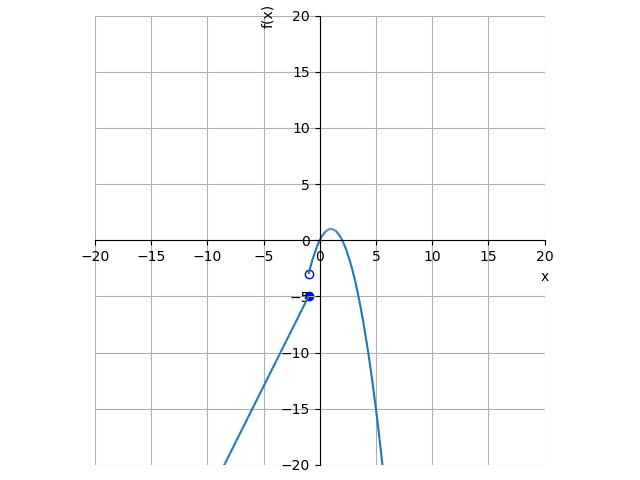
\includegraphics[width=1\columnwidth]{ex_funcion_a_trozos_2}}\end{solution} \part[1] $f(x)=\begin{cases} 3 - 2 x & \text{for}\: x < 1 \\- x^{2} + 6 x - 8 & \text{otherwise} \end{cases}$\begin{solution} \scalebox{.6}{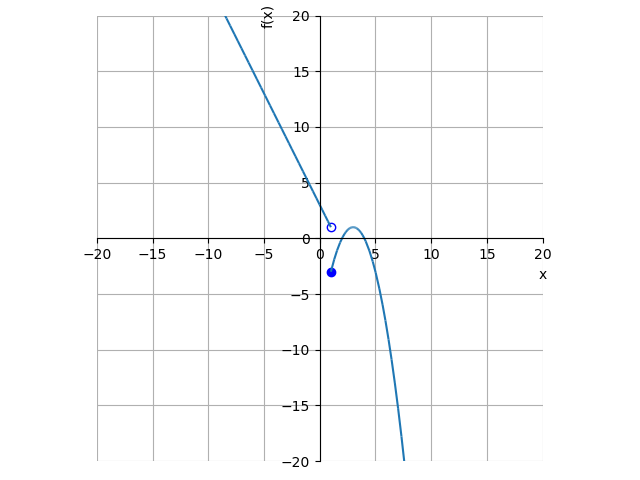
\includegraphics[width=1\columnwidth]{ex_funcion_a_trozos_3}}\end{solution} \part[1] $f(x)=\begin{cases} 2 x + 3 & \text{for}\: x < -2 \\3 & \text{for}\: x \leq 2 \\3 - x & \text{otherwise} \end{cases}$\begin{solution} \scalebox{.6}{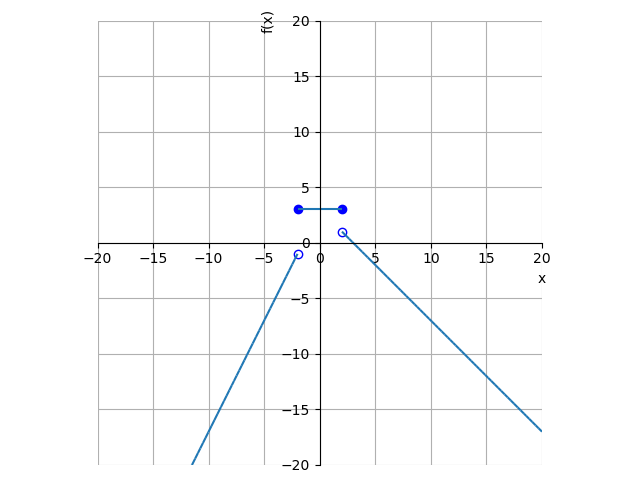
\includegraphics[width=1\columnwidth]{ex_funcion_a_trozos_4}}\end{solution} \part[1] $f(x)=\begin{cases} 3 - 2 x & \text{for}\: x < -1 \\3 & \text{for}\: x \leq 3 \\x + 3 & \text{otherwise} \end{cases}$\begin{solution} \scalebox{.6}{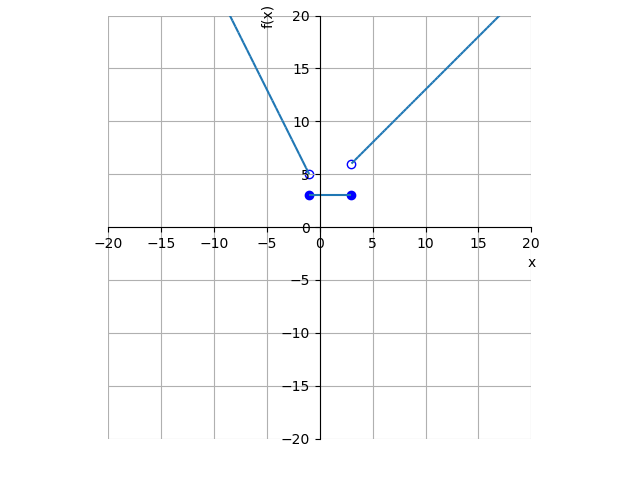
\includegraphics[width=1\columnwidth]{ex_funcion_a_trozos_5}}\end{solution} \part[1] $f(x)=\begin{cases} 2 x - 4 & \text{for}\: x < -2 \\- x^{2} + 4 x - 3 & \text{for}\: x < 3 \\3 & \text{for}\: x > 3 \end{cases}$\begin{solution} \scalebox{.6}{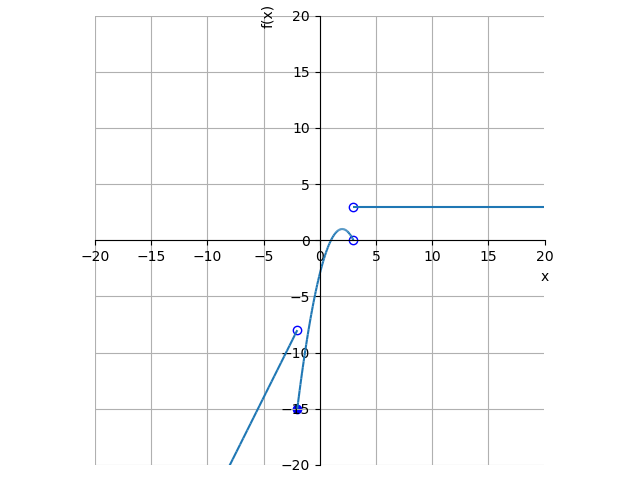
\includegraphics[width=1\columnwidth]{ex_funcion_a_trozos_6}}\end{solution} 
%\part[1] 
$$f(x)=\begin{cases} 4 - x & \text{for}\: x < -2 \\- x^{2} + 4 x - 3 & \text{for}\: x < 3 \\1 & \text{for}\: x > 3 \end{cases}$$\begin{solution} \scalebox{.6}{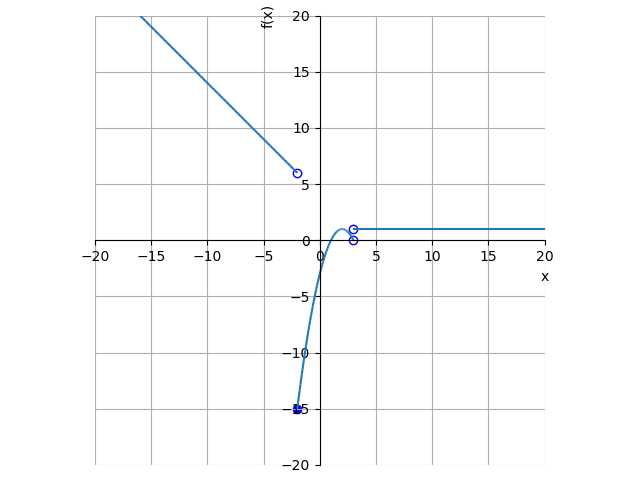
\includegraphics[width=1\columnwidth]{ex_funcion_a_trozos_7}}\end{solution} 
%\end{parts} 
 
 \question[1] Resuelve el siguiente sistema de inecuaciones:
 
 $$\left\{\begin{matrix}\dfrac{{x - 1}}{2} - \dfrac{{x + 2}}{3} \leq 12 \\  \dfrac{x}{2} - \dfrac{x}{3} \geq 3\end{matrix}\right.$$
\begin{solution} $\left[18, 79\right]$ \end{solution}
 
 \question[1] \textbf{Ejercicio postre:} Resuelve el siguiente sistema no lineal: $$\left\{\begin{matrix}x^2 + y^2 = 25 \\ xy+12=0\end{matrix}\right. $$
\begin{solution}
    $ \to \left[ \left\{ x = -4, \  y = 3\right\}, \  \left\{ x = -3, \  y = 4\right\}, \  \left\{ x = 3, \  y = -4\right\}, \  \left\{ x = 4, \  y = -3\right\}\right]$
\end{solution}

% \question[1] \textbf{Ejercicio postre:} Resuelve el siguiente sistema no lineal:$$\left\{\begin{matrix}3xy-4y^2=0 \\ 3x-2y=1\end{matrix}\right. $$\begin{solution}    $ \to \left[ \left\{ x = \frac{1}{3}, \  y = 0\right\}, \  \left\{ x = \frac{2}{3}, \  y = \frac{1}{2}\right\}\right]$\end{solution}

        
        
        
\section*{3ª Evaluación}    

\question[1]   Desde el lugar donde me encuentro la visual de la torre forma un ángulo de 32º con la
horizontal. Si me acerco 15 m, el ángulo es de 50º. ¿Cuál es la altura de la torre?
\begin{solution} $\left. \begin{gathered}
	  \tg 32 = \frac{y}{x} \\
	  \tg 50 = \frac{y}{x-15} \hfill
	 \end{gathered}  \right\rbrace \\
	 \to 
	 \frac{15 \tan{\left (\frac{8 \pi}{45} \right )} \tan{\left (\frac{5 \pi}{18} \right )}}{- \tan{\left (\frac{8 \pi}{45} \right )} + \tan{\left (\frac{5 \pi}{18} \right )}}\approx19.7048244137178 m $ \end{solution}
	 
	 \question[1] Calcula la recta $s$ que:\begin{parts} \part Pasa por el punto medio a P$\left( 1, \  -1\right)$ y  Q$\left( 5, \  3\right)$ y es perpendicular a $r \equiv 4 x - 2 y + 1 = 0$\begin{solution} $s\equiv y = \dfrac{5}{2} - \dfrac{x}{2}$\end{solution} \end{parts} 
	 
	 
	 \question[1] Resuelve las siguientes ecuaciones: \begin{parts} %\part[1] $\dfrac{1}{2}+\sin{x}=1$\begin{solution} $x=30^{\circ}, x=150^{\circ}$\end{solution} 
	 %\part[1] $\cos{x}-\dfrac{1}{4}=\dfrac{1}{4}$\begin{solution} $x=60^{\circ}, x=300^{\circ}$\end{solution} 
	 \part $(\cos{x})^2-\dfrac{1}{2}\cos{x}=0$\begin{solution} $x=60^{\circ}, x=90^{\circ}, x=270^{\circ}, x=300^{\circ}$\end{solution} 
	 \end{parts} 
	 
	 \question[1] Las calificaciones de un grupo de 26 alumnos han sido: 4 6 5 5 7 10 7 5 6 7 6 3 4 6 6 4 4 6 5 3 5 7 7 7 2 2. \begin{itemize} \item Realiza una tabla de frecuencias 
%	 \item Realiza un diagrama de barras 
	 \item Calcular la media y la mediana 
	 \item Calcular los parámetros de posición P70, Q1, Q3 
	% \item Calcular los parámetros de dispersión 
	 \item Realiza un diagrama de caja. \end{itemize}\begin{solution} $\begin{tabular}{rrrrrrr}
\hline
   $x_i$ &   $f_i$ &   $F_i$ &    $\%_i$ &   $\%A_i$ &   $x_if_i$ &   $x^2_if_i$ \\
\hline
       2 &       2 &       2 &   7.69231 &   7.69231 &          4 &            8 \\
       3 &       2 &       4 &   7.69231 &  15.3846  &          6 &           18 \\
       4 &       4 &       8 &  15.3846  &  30.7692  &         16 &           64 \\
       5 &       5 &      13 &  19.2308  &  50       &         25 &          125 \\
       6 &       6 &      19 &  23.0769  &  73.0769  &         36 &          216 \\
       7 &       6 &      25 &  23.0769  &  96.1538  &         42 &          294 \\
      10 &       1 &      26 &   3.84615 & 100       &         10 &          100 \\
     nan &      26 &     nan & 100       & nan       &        139 &          825 \\
\hline
\end{tabular}$\\ 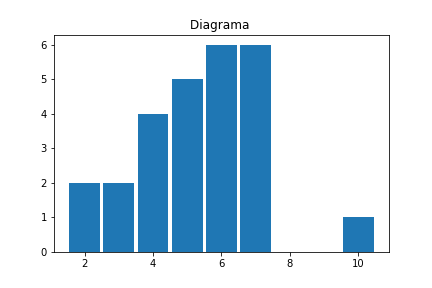
\includegraphics[width=0.7\columnwidth]{diagrama_exg2} \\ $\left\{ Me : 5.5, \  Mo : \left( [6], \  [6]\right), \  media : 5.35\right\}$ \\$\left\{ P70 : 6.0, \  Q1 : 4.0, \  Q3 : 6.75\right\}$ \\$\left\{ C.V : 0.33, \  desv.tip : 1.77, \  rango : 8, \  var : 3.15\right\}$\\ 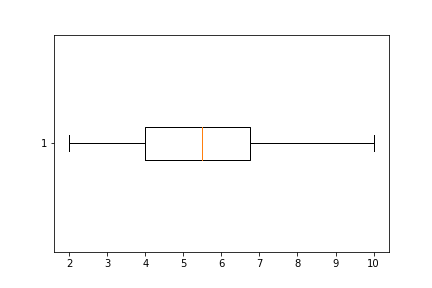
\includegraphics[width=0.7\columnwidth]{caja_exg2}\end{solution}


%\question[1] Las calificaciones de un grupo de 24 alumnos han sido: 6 5 5 7 10 7 5 6 7 3 4 8 8 4 4 6 5 3 5 7 7 7 2 2. \begin{itemize} \item Realiza una tabla de frecuencias \item Realiza un diagrama de barras \item Calcular los parámetros de centralización media, moda y mediana \item Calcular los parámetros de posición P70, Q1, Q3 \item Calcular los parámetros de dispersión varianza y desviación típica \item Realiza un diagrama de caja. \end{itemize}\begin{solution} $\begin{tabular}{rrrrrrr}
%\hline
%   $x_i$ &   $f_i$ &   $F_i$ &    $\%_i$ &   $\%A_i$ &   $x_if_i$ &   $x^2_if_i$ \\
%\hline
%       2 &       2 &       2 &   8.33333 &   8.33333 &          4 &            8 \\
%       3 &       2 &       4 &   8.33333 &  16.6667  &          6 &           18 \\
%       4 &       3 &       7 &  12.5     &  29.1667  &         12 &           48 \\
%       5 &       5 &      12 &  20.8333  &  50       &         25 &          125 \\
%       6 &       3 &      15 &  12.5     &  62.5     &         18 &          108 \\
%       7 &       6 &      21 &  25       &  87.5     &         42 &          294 \\
%       8 &       2 &      23 &   8.33333 &  95.8333  &         16 &          128 \\
%      10 &       1 &      24 &   4.16667 & 100       &         10 &          100 \\
%     nan &      24 &     nan & 100       & nan       &        133 &          829 \\
%\hline
%\end{tabular}$\\ 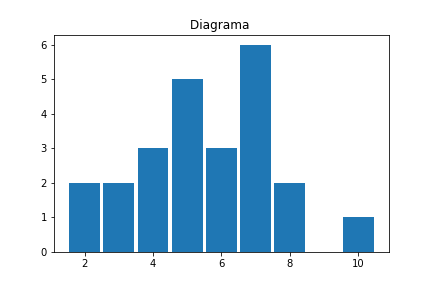
\includegraphics[width=0.7\columnwidth]{diagrama_exg3} \\ $\left\{ Me : 5.5, \  Mo : \left( [7], \  [6]\right), \  media : 5.54\right\}$ \\$\left\{ P70 : 7.0, \  Q1 : 4.0, \  Q3 : 7.0\right\}$ \\$\left\{ C.V : 0.35, \  desv.tip : 1.96, \  rango : 8, \  var : 3.83\right\}$\\ 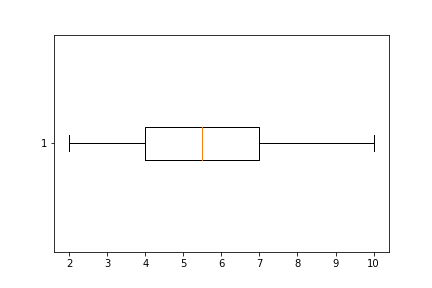
\includegraphics[width=0.7\columnwidth]{caja_exg3}\end{solution}
	 
	 \question[1] \textbf{Ejercicio postre:}  La diagonal menor de un rombo mide 20 cm y el ángulo menor es de 60º. ¿Cuánto mide la otra diagonal?¿Y el lado del rombo?\begin{solution} Miden $34.64$ y $20.0$ respectivamente\end{solution} 
     %La diagonal menor de un rombo mide 40 cm y el ángulo menor es de 60º. ¿Cuánto mide la otra diagonal?¿Y el lado del rombo?\begin{solution} Miden $69.28$ y $40.0$ respectivamente\end{solution}  
	 
	 
	 
        





        
    \end{questions}
    
    \newpage 
% [line cap=round,line join=round,>=triangle 45,x=1cm,y=1cm, scale=0.78]

\begin{tikzpicture}[x=1cm,y=1cm,scale=0.5]
\draw [color=lightgray,dash pattern=on 1pt off 1pt, xstep=1cm,ystep=1cm] (-10.1,-10.1) grid (10.1,10.1);
\draw[color=black] (-10.1,0) -- (10.1,0);
\foreach \x in {-10,-9,-8,-7,-6,-5,-4,-3,-2,-1,1,2,3,4,5,6,7,8,9,10}
\draw[shift={(\x,0)},color=black] (0pt,1pt) -- (0pt,-1pt) node[below] {\footnotesize $\x$};
\draw[color=black] (0,-10.43158220601634095) -- (0,10.1);
\foreach \y in {-10,-9,-8,-7,-6,-5,-4,-3,-2,-1,1,2,3,4,5,6,7,8,9,10}
\draw[shift={(0,\y)},color=black] (2pt,0pt) -- (-2pt,0pt) node[left] {\footnotesize $\y$};
\end{tikzpicture}

\begin{tikzpicture}[x=1cm,y=1cm,scale=0.5]
\draw [color=lightgray,dash pattern=on 1pt off 1pt, xstep=1cm,ystep=1cm] (-10.1,-10.1) grid (10.1,10.1);
\draw[color=black] (-10.1,0) -- (10.1,0);
\foreach \x in {-10,-9,-8,-7,-6,-5,-4,-3,-2,-1,1,2,3,4,5,6,7,8,9,10}
\draw[shift={(\x,0)},color=black] (0pt,1pt) -- (0pt,-1pt) node[below] {\footnotesize $\x$};
\draw[color=black] (0,-10.43158220601634095) -- (0,10.1);
\foreach \y in {-10,-9,-8,-7,-6,-5,-4,-3,-2,-1,1,2,3,4,5,6,7,8,9,10}
\draw[shift={(0,\y)},color=black] (2pt,0pt) -- (-2pt,0pt) node[left] {\footnotesize $\y$};
\end{tikzpicture}

    
    
%     \newgeometry{left=1 cm,bottom=2cm}
% \begin{landscape}
% \begin{table}[]
% \Large
% \centering
% \caption{Extracto de tabla de probabilidades de la \textbf{normal estándar $Z(0,1)$}}
% \label{my-label}

% \begin{tabular}{l|llllllllll}
% z   & 0       & 0,01    & 0,02    & 0,03    & 0,04    & 0,05    & 0,06    & 0,07    & 0,08    & 0,09    \\
% \hline
% 0   & 0,5     & 0,50399 & 0,50798 & 0,51197 & 0,51595 & 0,51994 & 0,52392 & 0,5279  & 0,53188 & 0,53586 \\
% 0,1 & 0,53983 & 0,5438  & 0,54776 & 0,55172 & 0,55567 & 0,55962 & 0,56356 & 0,56749 & 0,57142 & 0,57535 \\
% 0,2 & 0,57926 & 0,58317 & 0,58706 & 0,59095 & 0,59483 & 0,59871 & 0,60257 & 0,60642 & 0,61026 & 0,61409 \\
% 0,3 & 0,61791 & 0,62172 & 0,62552 & 0,6293  & 0,63307 & 0,63683 & 0,64058 & 0,64431 & 0,64803 & 0,65173 \\
% 0,4 & 0,65542 & 0,6591  & 0,66276 & 0,6664  & 0,67003 & 0,67364 & 0,67724 & 0,68082 & 0,68439 & 0,68793 \\
% 0,5 & 0,69146 & 0,69497 & 0,69847 & 0,70194 & 0,7054  & 0,70884 & 0,71226 & 0,71566 & 0,71904 & 0,7224  \\
% 0,6 & 0,72575 & 0,72907 & 0,73237 & 0,73565 & 0,73891 & 0,74215 & 0,74537 & 0,74857 & 0,75175 & 0,7549  \\
% 0,7 & 0,75804 & 0,76115 & 0,76424 & 0,7673  & 0,77035 & 0,77337 & 0,77637 & 0,77935 & 0,7823  & 0,78524 \\
% 0,8 & 0,78814 & 0,79103 & 0,79389 & 0,79673 & 0,79955 & 0,80234 & 0,80511 & 0,80785 & 0,81057 & 0,81327 \\
% 0,9 & 0,81594 & 0,81859 & 0,82121 & 0,82381 & 0,82639 & 0,82894 & 0,83147 & 0,83398 & 0,83646 & 0,83891 \\
% 1   & 0,84134 & 0,84375 & 0,84614 & 0,84849 & 0,85083 & 0,85314 & 0,85543 & 0,85769 & 0,85993 & 0,86214 \\
% %1,1 & 0,86433 & 0,8665  & 0,86864 & 0,87076 & 0,87286 & 0,87493 & 0,87698 & 0,879   & 0,881   & 0,88298 \\
% %1,2 & 0,88493 & 0,88686 & 0,88877 & 0,89065 & 0,89251 & 0,89435 & 0,89617 & 0,89796 & 0,89973 & 0,90147 \\
% %1,3 & 0,9032  & 0,9049  & 0,90658 & 0,90824 & 0,90988 & 0,91149 & 0,91309 & 0,91466 & 0,91621 & 0,91774 \\
% %1,4 & 0,91924 & 0,92073 & 0,9222  & 0,92364 & 0,92507 & 0,92647 & 0,92785 & 0,92922 & 0,93056 & 0,93189 \\
% %1,5 & 0,93319 & 0,93448 & 0,93574 & 0,93699 & 0,93822 & 0,93943 & 0,94062 & 0,94179 & 0,94295 & 0,94408 \\
% %1,6 & 0,9452  & 0,9463  & 0,94738 & 0,94845 & 0,9495  & 0,95053 & 0,95154 & 0,95254 & 0,95352 & 0,95449 \\
% %1,7 & 0,95543 & 0,95637 & 0,95728 & 0,95818 & 0,95907 & 0,95994 & 0,9608  & 0,96164 & 0,96246 & 0,96327 \\
% %1,8 & 0,96407 & 0,96485 & 0,96562 & 0,96638 & 0,96712 & 0,96784 & 0,96856 & 0,96926 & 0,96995 & 0,97062 \\
% %1,9 & 0,97128 & 0,97193 & 0,97257 & 0,9732  & 0,97381 & 0,97441 & 0,975   & 0,97558 & 0,97615 & 0,9767  \\
% %2   & 0,97725 & 0,97778 & 0,97831 & 0,97882 & 0,97932 & 0,97982 & 0,9803  & 0,98077 & 0,98124 & 0,98169 \\
% %2,1 & 0,98214 & 0,98257 & 0,983   & 0,98341 & 0,98382 & 0,98422 & 0,98461 & 0,985   & 0,98537 & 0,98574 \\
% %2,2 & 0,9861  & 0,98645 & 0,98679 & 0,98713 & 0,98745 & 0,98778 & 0,98809 & 0,9884  & 0,9887  & 0,98899 \\
% %2,3 & 0,98928 & 0,98956 & 0,98983 & 0,9901  & 0,99036 & 0,99061 & 0,99086 & 0,99111 & 0,99134 & 0,99158 \\
% %2,4 & 0,9918  & 0,99202 & 0,99224 & 0,99245 & 0,99266 & 0,99286 & 0,99305 & 0,99324 & 0,99343 & 0,99361 \\
% %2,5 & 0,99379 & 0,99396 & 0,99413 & 0,9943  & 0,99446 & 0,99461 & 0,99477 & 0,99492 & 0,99506 & 0,9952  \\
% %2,6 & 0,99534 & 0,99547 & 0,9956  & 0,99573 & 0,99585 & 0,99598 & 0,99609 & 0,99621 & 0,99632 & 0,99643 \\
% %2,7 & 0,99653 & 0,99664 & 0,99674 & 0,99683 & 0,99693 & 0,99702 & 0,99711 & 0,9972  & 0,99728 & 0,99736 \\
% %2,8 & 0,99744 & 0,99752 & 0,9976  & 0,99767 & 0,99774 & 0,99781 & 0,99788 & 0,99795 & 0,99801 & 0,99807 \\
% %2,9 & 0,99813 & 0,99819 & 0,99825 & 0,99831 & 0,99836 & 0,99841 & 0,99846 & 0,99851 & 0,99856 & 0,99861 \\
% %3   & 0,99865 & 0,99869 & 0,99874 & 0,99878 & 0,99882 & 0,99886 & 0,99889 & 0,99893 & 0,99896 & 0,999   \\
% %3,1 & 0,99903 & 0,99906 & 0,9991  & 0,99913 & 0,99916 & 0,99918 & 0,99921 & 0,99924 & 0,99926 & 0,99929 \\
% %3,2 & 0,99931 & 0,99934 & 0,99936 & 0,99938 & 0,9994  & 0,99942 & 0,99944 & 0,99946 & 0,99948 & 0,9995  \\
% %3,3 & 0,99952 & 0,99953 & 0,99955 & 0,99957 & 0,99958 & 0,9996  & 0,99961 & 0,99962 & 0,99964 & 0,99965 \\
% %3,4 & 0,99966 & 0,99968 & 0,99969 & 0,9997  & 0,99971 & 0,99972 & 0,99973 & 0,99974 & 0,99975 & 0,99976 \\
% %3,5 & 0,99977 & 0,99978 & 0,99978 & 0,99979 & 0,9998  & 0,99981 & 0,99981 & 0,99982 & 0,99983 & 0,99983 \\
% %3,6 & 0,99984 & 0,99985 & 0,99985 & 0,99986 & 0,99986 & 0,99987 & 0,99987 & 0,99988 & 0,99988 & 0,99989 \\
% %3,7 & 0,99989 & 0,9999  & 0,9999  & 0,9999  & 0,99991 & 0,99991 & 0,99992 & 0,99992 & 0,99992 & 0,99992 \\
% %3,8 & 0,99993 & 0,99993 & 0,99993 & 0,99994 & 0,99994 & 0,99994 & 0,99994 & 0,99995 & 0,99995 & 0,99995 \\
% %3,9 & 0,99995 & 0,99995 & 0,99996 & 0,99996 & 0,99996 & 0,99996 & 0,99996 & 0,99996 & 0,99997 & 0,99997 \\
% %4   & 0,99997 & 0,99997 & 0,99997 & 0,99997 & 0,99997 & 0,99997 & 0,99998 & 0,99998 & 0,99998 & 0,99998
% \end{tabular}
% \end{table}
% \end{landscape}
% \restoregeometry
    \end{document}
    
